\documentclass[a4paper,twoside,master.tex]{subfiles}
\begin{document}
\lecture{19}{Wednesday, February 26, 2020}{Extremum Principles, Continued}

\begin{figure}[h]
    \centering
    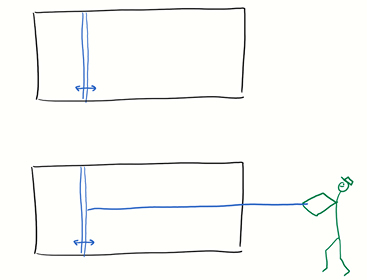
\includegraphics[width=\textwidth]{figures/lec_19_piston.png}
    \caption{Top: A constraint being released, changing the entropy.\\Bottom: A constraint being released adiabatically, leaving the entropy constant.\\Credit: Logan Carpenter}
    \label{fig:lec_19_piston}
\end{figure}

In the top image of \Cref{fig:lec_19_piston}, the process which moves the wall to a new equilibrium state is irreversible. The energy stays constant and the entropy increases, and at the new equilibrium, $ \eval{\pdv{S}{x}}_{U} = 0 $ and $ \eval{\pdv[2]{S}{x}}_{U} < 0 $. In the bottom image, we perform the same process adiabatically such that the entropy stays the same while the energy changes. We will show that the energy has reached a new minimum. In the top image, we can take a total derivative of the entropy to first order:
\begin{equation}
    \dd{S} = \underbrace{\eval{\pdv{S}{U}}_{x}}_{\frac{1}{T}} \dd{U} + \underbrace{\eval{\pdv{S}{X}}_{U}}_{0} \dd{X}
\end{equation}
Let's write the next-order expansion in $ x $. Typically we don't do this, but since all the interesting stuff vanished at first-order, it might be important:
\begin{equation}
    \dd{S} = \underbrace{\eval{\pdv{S}{U}}_{x}}_{\frac{1}{T}} \dd{U} + \underbrace{\eval{\pdv{S}{X}}_{U}}_{0} \dd{X} + \frac{1}{2} \underbrace{\eval{\pdv[2]{S}{x}}_{U}}_{<0} (\dd{X})^2
\end{equation}

What happens in the second case? Rewriting the previous equation in terms of $ \dd{U} $, we see that
\begin{alignat}{3}
    \dd{U} &= T \dd{S} &&+ 0 \vdot \dd{x} &&- \frac{1}{2} T \eval{\pdv[2]{S}{x}}_{U} (\dd{x})^2 \\
    &= \eval{\pdv{U}{S}}_{x} \dd{S} &&+ \eval{\pdv{U}{x}}_{S} \dd{x} &&+ \frac{1}{2} \eval{\pdv[2]{U}{x}}_{S} (\dd{x})^2
\end{alignat}
where the second line is again the total derivative of $ U $ expanded to second order in $ x $. We can identify the terms (the differentials) to show that
\begin{equation}
    \eval{\pdv{U}{x}}_{S} = 0 \qquad \eval{\pdv[2]{U}{x}}_{S} > 0
\end{equation}
for the second scenario. \textit{At constant entropy, the total energy is minimized in thermal equilibrium.}


What if the system is at constant $ T $? Imagine we put the adiabatic system in contact with a reservoir at constant temperature $ T_R $? This entire system, reservoir and original system combined, is equivalent to the second system. Energy must be minimized, so the principles of the second case apply to the total combined energy of both subsystems (calling the reservoir energy $ U_R $):
\begin{align}
    \text{In equilibrium} &\begin{cases} \pdv{x}(U + U_R) = 0 & (1)\\ \pdv[2]{x}(U + U_R) > 0 & (2)  \end{cases}\\
    S+S_R &= \text{ const. } \forall x \qquad (3)
\end{align}
Since the reservoir interacts with the system only via heat exchange,
\begin{align}
    \dd{U_R} &= \underbrace{\dbar{W_R}}_{0} + \dbar{Q_R} = T_R \dd{S_R} \\
    & \implies \pdv{U_R}{x} = T_R \pdv{S_R}{x} \qquad (4)
\end{align}

Since our system is at constant $ \{T,V,N\} $, let's consider the change in Helmholtz free energy in equilibrium (the free energy of the system alone, not the system and reservoir combined):
\begin{align}
    \pdv{F}{x} &= \pdv{x} (U - TS) \\
    &= \pdv{U}{x} - T \pdv{S}{x} \\
    &= \pdv{U}{x} - T_R \pdv{S}{x}
\end{align}
since the system is in thermal equilibrium with the reservoir (so $ T = T_R $).
\begin{align}
    \pdv{F}{x} &= \pdv{U}{x} + T_R \pdv{S_R}{x} \qq{by} (3) \\
    &= \pdv{U}{x} + \pdv{U_R}{x} \qq{by} (4) \\
    &= \pdv{x}(U + U_R) = 0 \qq{by} (1)
\end{align}
Therefore, we have reached an extremum in $ F $ at equilibrium. Is it a maximum or a minimum? We can go through all of these same steps again at a second derivative level and use equation $ (2) $ to show that
\begin{equation}
    \pdv[2]{F}{x} > 0
\end{equation}

Therefore, at constant $ \{T,V,N\} $, the Helmholtz free energy $ F $ is at a minimum at equilibrium. Notice the pattern here. $ F(T,V,N) $ is minimized when $ T $, $ V $, and $ N $ are fixed. When $ S $, $ V $, and $ N $ are constant, $ U(S,V,N) $ is minimized. The only exception is that $ S(U,V,N) $ is maximized when $ U $, $ V $, and $ N $ are fixed. Similar extremum principles can be derived for the other thermodynamic potentials.


Recall that
\begin{equation}
    \dd{F} = -S \dd{T} - P \dd{V} + \mu \dd{N}
\end{equation}
At constant $ T $ and $ N $,
\begin{equation}
    \dd{F} = - P \dd{V} = \dbar{W}
\end{equation}

The maximum work that can be extracted at constant $ T $, $ V $, and $ N $ is the change in free energy between initial and final state. Similarly, if the entropy is constant, the energy $ U $ determines the maximum work that can be extracted. Note that when we say $ V $ is constant, we are talking about the volume of the system as a whole, so $ P \dd{V} $ is not zero, as this refers to the rearrangement of volumes inside the system.


For a final example, consider a system at constant $ T $, $ P $, and $ \{N_i\} $ (multiple species of particles, although this is not important, but it's good to know how to deal with this).
\begin{equation}
    \dd{G} = - S \dd{T} + V \dd{P} + \sum_i \mu_i \dd{N_i}
\end{equation}
If the pressure is fixed, what happens? There is now work being done on the system to keep the pressure constant (in addition to heat being exchanged to keep the temperature constant). We can realize this by the system plus a $ T $-reservoir plus a ``$ P $-reservoir'' at constant energy:
\begin{align}
    \pdv{x}(U + U_R) &= 0\quad \text{at equilibrium} \qquad (1)\\
    \pdv[2]{x}(U + U_R) &> 0\quad \text{at equilibrium} \qquad (2) \\
    S + S_R &= \text{const.}\quad \forall x \qquad (3) \\
    V + V_R &= \text{const.}\quad \forall x \qquad (4) \\
    \dd{U_R} = T_R \dd{S_R} - P_R \dd{V_R} \qquad (5)
\end{align}
\begin{align}
    \dv{G}{x} &= \pdv{x}(U - TS + PV) \\
    &= \pdv{x}U - T_R \pdv{S}{x} + P_R \pdv{V}{x} \\
    &= \pdv{x}U \underbrace{+ T_R \pdv{S_R}{x}}_{(3)} \underbrace{- P_R \pdv{V_R}{x}}_{(4)} \\
    &= \pdv{U}{x} \underbrace{\pdv{U_R}{x}}_{(5)} = \pdv{x}(U + U_R) \underbrace{= 0}_{(1)}
\end{align}
Additionally, we can do the same thing to show that in this situation, $ \pdv[2]{G}{x} > 0 $ using equation $ (2) $. We can do similar things with the grand potential and the enthalpy, which all have dimension of energy. The only odd-one-out is the entropy, which does not have energy units.

\end{document}
